\heading{群论I-zy-25秋-期末}

\begin{question}[8 分]
证明：魔方(右图玩具)的所有可行操作(可多步)构成一个群，并判断其是否为 Abel 群。
\begin{center}
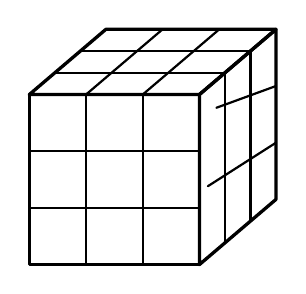
\begin{tikzpicture}[scale=0.72,line join=round,line cap=round]
  % Isometric 3x3 cube: three faces share only boundary vertices; all grid lines are clipped to a face.
  \coordinate (O) at (0,0);
  \coordinate (X) at (3,0);
  \coordinate (Y) at (0,3);
  \coordinate (T) at (1.35,1.15);
  \coordinate (XT) at (4.35,1.15);
  \coordinate (YT) at (1.35,4.15);
  \coordinate (XY) at (3,3);
  \coordinate (XYT) at (4.35,4.15);
  % front, right, top outlines
  \draw[very thick] (O)--(X)--(XY)--(Y)--cycle;
  \draw[very thick] (X)--(XT)--(XYT)--(XY)--cycle;
  \draw[very thick] (Y)--(XY)--(XYT)--(YT)--cycle;
  % front grid
  \foreach \a in {1,2}{\draw[thick] (\a,0)--(\a,3); \draw[thick] (0,\a)--(3,\a);}
  % right face: affine interpolation
  \foreach \a in {1,2}{
    \draw[thick] ({3+0.45*\a},{0+1.15*\a/3})--({3+0.45*\a},{3+1.15*\a/3});
    \draw[thick] ({3+0.45*\a/3},{\a+1.15*\a/3})--({4.35},{\a+1.15});
  }
  % top face
  \foreach \a in {1,2}{
    \draw[thick] ({0+0.45*\a},{3+1.15*\a/3})--({3+0.45*\a},{3+1.15*\a/3});
    \draw[thick] (\a,3)--({\a+1.35},4.15);
  }
\end{tikzpicture}
\end{center}
\begin{solution}
把每个可行操作看作对魔方所有可动小块(连同其朝向)的一个置换。若 $g,h$ 都是可行操作，则先作 $h$ 再作 $g$ 的复合 $gh$ 仍是有限步转动，因而仍可行，故封闭。操作复合继承函数复合的结合律。什么也不做给出单位元 $e$。任一基本转动都可反向转回，因此任意有限步操作的逆操作按相反次序逐步撤销，仍是可行操作。故所有可行操作构成群。

它不是 Abel 群。例如记 $R$ 为右面顺时针转 $90^\circ$，$U$ 为上面顺时针转 $90^\circ$。角块 $URF$ 在 $RU$ 与 $UR$ 下最终位置(以及朝向)不同，因此
\[
RU\neq UR.
\]
所以
\[
\boxed{\text{魔方群是非 Abel 群}}.
\]
\end{solution}
\end{question}

\begin{question}[9 分]
求六阶置换群 $S_6$ 中群元 $g$ 的轮换结构、杨图和 $g$ 的阶数：
\[
g=\begin{pmatrix}
1&2&3&4&5&6\\
3&4&6&2&1&5
\end{pmatrix}.
\]
\begin{solution}
从 $1$ 开始追踪：
\[
1\to3\to6\to5\to1,
\]
得到四轮换 $(1\,3\,6\,5)$；余下
\[
2\to4\to2,
\]
得到二轮换 $(2\,4)$。故
\[
\boxed{g=(1\,3\,6\,5)(2\,4)}.
\]
轮换型为分拆
\[
\boxed{6=4+2},
\]
其杨图为两行，行长分别为 $4$ 与 $2$：
\[
\boxed{[4,2]}
\]
群元阶为各互不相交轮换长度的最小公倍数：
\[
\boxed{\operatorname{ord}(g)=\operatorname{lcm}(4,2)=4}.
\]
\end{solution}
\end{question}

\begin{question}[8 分]
求以下分子的点群(Schoenflies 符号)和其各共轭类下包含的对称性操作：
\[
[\mathrm{PdCl_4}]^{2-}.
\]
\begin{center}
\begin{tikzpicture}[line cap=round,line join=round]
  \begin{scope}[xshift=-2.5cm]
    \node[font=\small\bfseries] at (0,2.15) {正面};
    \draw[thick] (-1.15,0)--(1.15,0) (0,-1.15)--(0,1.15);
    \node[draw,circle,minimum size=8mm] at (0,0) {Pd};
    \foreach \x/\y in {1.35/0,-1.35/0,0/1.35,0/-1.35}{\node[draw,circle,minimum size=7mm] at (\x,\y) {Cl};}
  \end{scope}
  \begin{scope}[xshift=2.5cm]
    \node[font=\small\bfseries] at (0,2.15) {侧面};
    \draw[thick] (0,-1.15)--(0,1.15);
    \node[draw,circle,minimum size=8mm] at (0,0) {Pd};
    \node[draw,circle,minimum size=7mm] at (0,1.35) {Cl};
    \node[draw,circle,minimum size=7mm] at (0,-1.35) {Cl};
    \node[font=\scriptsize,align=center] at (0,-2.05) {其余两只 Cl 沿视线方向重合};
  \end{scope}
\end{tikzpicture}
\end{center}
\begin{solution}
该离子为方平面构型。取分子平面为 $xy$ 平面，$z$ 轴垂直分子平面，则主轴为 $C_4$，并有分子平面 $\sigma_h$、反演中心 $i$、两类面内二重轴以及两类竖直镜面，故
\[
\boxed{[\mathrm{PdCl_4}]^{2-}:D_{4h}}.
\]
$D_{4h}$ 的十个共轭类及其元素可列为
\[
\begin{array}{c|l}
\text{共轭类}&\text{对称操作}\\\hline
E&\{E\}\\
2C_4&\{C_4,C_4^3\}\\
C_2&\{C_4^2\}\\
2C_2'&\{C_{2x},C_{2y}\}\\
2C_2''&\{C_{2,\,x=y},C_{2,\,x=-y}\}\\
i&\{i\}\\
2S_4&\{S_4,S_4^3\}\\
\sigma_h&\{\sigma_h\}\\
2\sigma_v&\{\sigma_{xz},\sigma_{yz}\}\\
2\sigma_d&\{\sigma_{x=y},\sigma_{x=-y}\}
\end{array}
\]
总元素数 $1+2+1+2+2+1+2+1+2+2=16$，与 $|D_{4h}|=16$ 一致。
\end{solution}
\end{question}

\begin{question}[9 分]
求下列 $D_3$ 群特征标表中特征标第一、二正交定理和 Burnside 定理的体现：
\[
\begin{array}{c|ccc}
D_3&\{E\}&2\{C_3\}&3\{C_2\}\\\hline
A_1&1&1&1\\
A_2&1&1&-1\\
A_3&2&-1&0
\end{array}
\]
\begin{solution}
$D_3$ 的阶为 $6$，三类大小分别为 $1,2,3$。

第一正交定理(不同行正交)为
\[
\frac1{6}\left[
\chi_\alpha(E)^*\chi_\beta(E)
+2\chi_\alpha(C_3)^*\chi_\beta(C_3)
+3\chi_\alpha(C_2)^*\chi_\beta(C_2)
\right]=\delta_{\alpha\beta}.
\]
例如
\[
\frac16[1\cdot2+2(1)(-1)+3(1)(0)]=0,
\]
说明 $A_1$ 与 $A_3$ 正交；每一行的自内积都等于 $1$。

第二正交定理(不同类的列正交)给出
\[
\sum_\alpha \chi_\alpha(C)^*\chi_\alpha(C')=0\qquad(C\neq C'),
\]
而同一类满足
\[
\sum_\alpha|\chi_\alpha(C)|^2=\frac{|G|}{|C|}.
\]
在表中分别为
\[
1^2+1^2+2^2=6,\qquad
1^2+1^2+(-1)^2=3,\qquad
1^2+(-1)^2+0^2=2,
\]
恰好等于 $6/1,6/2,6/3$。

Burnside 完备性关系表现为不可约表示维数平方和等于群阶：
\[
\boxed{1^2+1^2+2^2=6=|D_3|}.
\]
\end{solution}
\end{question}

\begin{question}[8 分]
求六阶循环群 $Z_6$ 同态于 $Z_2$ 群的同态核，并给出可依此得到的 $Z_6$ 群的不可约表示。
\begin{solution}
设 $Z_6=\langle a\rangle$，$Z_2=\{\bar0,\bar1\}$。非平凡同态由
\[
\varphi(a)=\bar1
\]
唯一确定，于是
\[
\varphi(a^k)=\bar k\pmod2.
\]
其核为偶次幂：
\[
\boxed{\ker\varphi=\{e,a^2,a^4\}=\langle a^2\rangle\cong Z_3}.
\]
第一同构定理给出
\[
Z_6/\ker\varphi\cong Z_2,
\]
从而得到一个非平凡一维表示
\[
\chi_{\mathrm{par}}(a^k)=(-1)^k.
\]
再结合核 $Z_3$ 的三个一维特征标，就得到 $Z_6\cong Z_2\times Z_3$ 的全部六个不可约表示：
\[
\boxed{\chi_\ell(a^k)=\exp\!\left(\frac{2\pi\ii\ell k}{6}\right)},
\qquad \ell=0,1,\ldots,5.
\]
\end{solution}
\end{question}

\begin{question}[8 分]
三个($i=1,2,3$)两能级($p_i=+,-$)粒子的波函数
$\psi_{p_1}^{(1)}\psi_{p_2}^{(2)}\psi_{p_3}^{(3)}$ 空间中，求玻色统计全同粒子所允许(承载置换群 $S_3$ 的一维恒等表示 $\Gamma_1^s$)的基函数，并给出推理过程。
\begin{solution}
单粒子内部空间为二维，三粒子空间为 $(\mathbb C^2)^{\otimes3}$。玻色子要求对任意置换 $P\in S_3$ 都满足
\[
P\Psi=\Psi,
\]
即取完全对称子空间 $\operatorname{Sym}^3(\mathbb C^2)$。其维数为
\[
\binom{2+3-1}{3}=4.
\]
一组规范正交基为
\[
\boxed{|+++\rangle},
\qquad
\boxed{|---\rangle},
\]
\[
\boxed{\frac1{\sqrt3}\bigl(|-++\rangle+|+-+\rangle+|++-\rangle\bigr)},
\]
\[
\boxed{\frac1{\sqrt3}\bigl(|+--\rangle+|-+-\rangle+|--+\rangle\bigr)}.
\]
每个态都在 $S_3$ 的全部置换下不变，因此承载恒等表示 $\Gamma_1^s$。
\end{solution}
\end{question}

\begin{question}[10 分]
空间群的点群为 $C_{4h}$ 群的简单四方晶体，求第一布里渊区中的不可约布里渊区(可画图)，以及承载一维恒等表示的初态电偶极跃迁所允许末态的不可约表示。
\begin{solution}
简单四方倒格子仍为简单四方格子。若实空间晶格常数为 $a,a,c$，第一布里渊区可写成
\[
-\frac{\pi}{a}\le k_x,k_y\le\frac{\pi}{a},
\qquad
-\frac{\pi}{c}\le k_z\le\frac{\pi}{c}.
\]
$C_{4h}=\langle C_{4z},\sigma_h\rangle$ 的作用包括绕 $z$ 轴的四重转动以及 $k_z\mapsto-k_z$。因此一个方便的基本域可取
\[
\boxed{0\le k_x\le\frac{\pi}{a},\quad
0\le k_y\le\frac{\pi}{a},\quad
0\le k_z\le\frac{\pi}{c}}.
\]
它占整个第一布里渊区体积的 $1/8$。由于 $C_{4h}$ 本身没有竖直镜面，不能再用 $k_x\leftrightarrow k_y$ 把底面缩成三角形。

电偶极算符按极向量变换。对 $C_{4h}$ 的通常实表示记号，
\[
z\sim A_u,\qquad (x,y)\sim E_u.
\]
初态为全对称的一维恒等表示 $A_g$。电偶极矩阵元非零要求
\[
\Gamma_f\subset \Gamma_{\mathbf r}\otimes\Gamma_i=\Gamma_{\mathbf r},
\]
因此允许的末态为
\[
\boxed{A_u\ \text{($z$ 偏振)}},\qquad
\boxed{E_u\ \text{($x,y$ 偏振)}}.
\]
若坚持在复数域把 Abel 群 $C_{4h}$ 的表示完全拆成一维表示，则 $E_u$ 等价于一对互为复共轭、$C_4$ 本征值为 $\pm\ii$ 的一维表示。
\end{solution}
\end{question}

\begin{question}[10 分]
求 $SO(3)$ 群中转轴为 $z$ 方向、转角为 $\phi$ 的群元 $C_{\hat z}(\phi)$ 在三维实空间 $\mathbb R^3$ 和二次齐次函数 $x^2,y^2,z^2,xy,xz,yz$ 的线性空间上的表示矩阵和特征标。
\begin{solution}
记 $c=\cos\phi$，$s=\sin\phi$。在基 $(x,y,z)$ 上，
\[
D^{(1)}(C_{\hat z}(\phi))=
\begin{pmatrix}
c&-s&0\\
s&c&0\\
0&0&1
\end{pmatrix},
\qquad
\boxed{\chi^{(1)}(\phi)=1+2\cos\phi}.
\]

在基
\[
\mathcal B=(x^2,y^2,z^2,xy,xz,yz)
\]
上用
\[
x\mapsto cx-sy,\qquad y\mapsto sx+cy,\qquad z\mapsto z
\]
逐项展开，得到
\[
D^{(2)}(\phi)=
\begin{pmatrix}
c^2&s^2&0&cs&0&0\\
s^2&c^2&0&-cs&0&0\\
0&0&1&0&0&0\\
-2cs&2cs&0&c^2-s^2&0&0\\
0&0&0&0&c&s\\
0&0&0&0&-s&c
\end{pmatrix}.
\]
取迹：
\[
\chi^{(2)}=2c^2+1+(c^2-s^2)+2c
=\boxed{2+2\cos\phi+2\cos2\phi}.
\]
\end{solution}
\end{question}

\begin{question}[10 分]
求 $D_2$ 群在其群代数上的左正则表示，并通过特征标投影算符构造其群代数上承载各不等价不可约表示的对称化基函数(如需特征标表可自行推导)。
\begin{solution}
写成 Klein 四元群
\[
D_2=\{e,a,b,c\},\qquad a^2=b^2=c^2=e,\qquad ab=c.
\]
在群代数基 $(|e\rangle,|a\rangle,|b\rangle,|c\rangle)$ 上，左乘给出
\[
L_e=I_4,
\]
\[
L_a=\begin{pmatrix}0&1&0&0\\1&0&0&0\\0&0&0&1\\0&0&1&0\end{pmatrix},\quad
L_b=\begin{pmatrix}0&0&1&0\\0&0&0&1\\1&0&0&0\\0&1&0&0\end{pmatrix},\quad
L_c=\begin{pmatrix}0&0&0&1\\0&0&1&0\\0&1&0&0\\1&0&0&0\end{pmatrix}.
\]
$D_2$ 为 Abel 群，因此有四个一维不可约表示。可取特征标
\[
\begin{array}{c|rrrr}
&e&a&b&c\\\hline
A&1&1&1&1\\
B_1&1&1&-1&-1\\
B_2&1&-1&1&-1\\
B_3&1&-1&-1&1
\end{array}
\]
特征标投影算符为
\[
P_\alpha=\frac14\sum_{g\in D_2}\chi_\alpha(g)^*L_g.
\]
作用于 $|e\rangle$ 并归一化，得到
\[
\boxed{|A\rangle=\frac12(|e\rangle+|a\rangle+|b\rangle+|c\rangle)},
\]
\[
\boxed{|B_1\rangle=\frac12(|e\rangle+|a\rangle-|b\rangle-|c\rangle)},
\]
\[
\boxed{|B_2\rangle=\frac12(|e\rangle-|a\rangle+|b\rangle-|c\rangle)},
\]
\[
\boxed{|B_3\rangle=\frac12(|e\rangle-|a\rangle-|b\rangle+|c\rangle)}.
\]
四个对称化基函数互相正交，并恰好分解四维左正则表示。
\end{solution}
\end{question}

\begin{question}[10 分]
由 $C_4$ 群的一维非恒等表示
\[
A(C_4^k)=\ee^{2\pi\ii k/4}
\]
诱导出 $D_4$ 群的某表示，并展示此表示不可约且满足 Frobenius 定理。
\begin{solution}
令
\[
D_4=\langle r,s\mid r^4=e,\ s^2=e,\ srs=r^{-1}\rangle,
\qquad H=\langle r\rangle=C_4.
\]
给定 $H$ 上的特征标 $\chi(r^k)=\ii^k$。因为 $[D_4:H]=2$，诱导表示为二维。取陪集代表 $\{e,s\}$，可选基使
\[
\Gamma(r)=\begin{pmatrix}\ii&0\\0&-\ii\end{pmatrix},
\qquad
\Gamma(s)=\begin{pmatrix}0&1\\1&0\end{pmatrix}.
\]
因此
\[
\chi_\Gamma(e)=2,\quad
\chi_\Gamma(r^2)=-2,\quad
\chi_\Gamma(r)=\chi_\Gamma(r^3)=0,
\]
并且四个反射元的特征标均为 $0$。这是 $D_4$ 的标准二维不可约表示 $E$。

用特征标内积检验：
\[
\langle\chi_\Gamma,\chi_\Gamma\rangle
=\frac18\left(|2|^2+|-2|^2\right)=1,
\]
所以诱导表示不可约。

Frobenius 互反律为
\[
\left\langle\operatorname{Ind}_{C_4}^{D_4}\chi,\ E\right\rangle_{D_4}
=\left\langle\chi,\operatorname{Res}_{C_4}^{D_4}E\right\rangle_{C_4}.
\]
限制 $E$ 到 $C_4$ 后
\[
\Gamma(r)=\operatorname{diag}(\ii,-\ii),
\]
故
\[
\operatorname{Res}_{C_4}^{D_4}E=\chi\oplus\chi^*,
\]
右边内积为 $1$；左边也为 $1$，与诱导结果一致。
\end{solution}
\end{question}

\begin{question}[10 分]
引入自旋轨道耦合后，系统对称性从轨道的 $D_3$ 群(特征标表见第 4 题)与自旋的 $SU(2)$ 群直积群降低到双群 $D_3^D$。其特征标表如下，求由此导致的能级劈裂。请考虑承载 $D_3$ 群各不可约表示的初始态。
\[
\begin{array}{c|rrrrrr}
D_3^D&E&\bar E&2C_3&2\bar E C_3&3C_2^{(1)}&3\bar E C_2^{(1)}\\\hline
\Gamma_1&1&1&1&1&1&1\\
\Gamma_2&1&1&1&1&-1&-1\\
\Gamma_3&2&2&-1&-1&0&0\\
\Gamma_4&2&-2&1&-1&0&0\\
\Gamma_5&1&-1&-1&1&\ii&-\ii\\
\Gamma_6&1&-1&-1&1&-\ii&\ii
\end{array}
\]
\begin{solution}
$D_3$ 的单值轨道不可约表示分别对应双群表中的
\[
A_1\leftrightarrow\Gamma_1,\qquad
A_2\leftrightarrow\Gamma_2,\qquad
E\leftrightarrow\Gamma_3.
\]
原卷第 4 题把二维表示记作 $A_3$；按常用 Schoenflies 记号它就是这里的二维表示 $E$。
自旋 $1/2$ 在转角 $\theta$ 下的特征标为 $2\cos(\theta/2)$，而 $2\pi$ 转动作用为 $-I$。因此其限制到 $D_3^D$ 的特征标为
\[
(2,-2,1,-1,0,0),
\]
即
\[
\boxed{\Gamma_{1/2}=\Gamma_4}.
\]
于是逐个作直积：
\[
\Gamma_1\otimes\Gamma_4=\Gamma_4,
\qquad
\Gamma_2\otimes\Gamma_4=\Gamma_4.
\]
对二维轨道态，特征标逐类相乘得到
\[
\chi_{\Gamma_3\otimes\Gamma_4}=(4,-4,-1,1,0,0).
\]
与表中各行比较可得
\[
\boxed{\Gamma_3\otimes\Gamma_4
=\Gamma_4\oplus\Gamma_5\oplus\Gamma_6}.
\]
因此：
\begin{itemize}
  \item 原来轨道 $A_1$ 或 $A_2$ 的非简并能级，乘上自旋二重简并后都形成一个 $\Gamma_4$ 双群二重态；
  \item 原来轨道 $E$ 的二重简并态连同自旋共有四维，SOC 后分裂为一个二维 $\Gamma_4$ 与两个一维双值表示 $\Gamma_5,\Gamma_6$。
\end{itemize}
若系统还保持时间反演对称且无磁场，Kramers 定理要求 $\Gamma_5$ 与 $\Gamma_6$ 互为共轭并成对简并，因此物理能谱通常表现为两个 Kramers 双重能级。
\end{solution}
\end{question}
